\section{Upside Down Chamber}

\margininbox{\footnotesize{Upside Down Chamber}}{
		\begin{citemize}
		\item Rhys Tyers
		\item Arun Paul
		\end{citemize}}{\explo}

Awww, Arun's first pushing trip. We'd made good time to the end of exploration. A passage, \passage{Colony} intersected a large chamber. The chamber was split into two sections. A shaft dropped directly beneath us, Tanguy and Jack had been down there before, reporting there was still a lead. Rising up halfway up the height of the chamber a wall split the shaft from the rest of the huge space. A steep boulder slope descended on the other side.

It was an intimidating pitch. Arun was clearly quite nervous and I was a little giddy from a heady mix of excitement and fear. Descending it also becomes clear the the final part of the floor of the passage we were in is in fact jammed boulders above the pitch. I asked Arun to try not to move too much.

Tanguy had pulled the rope up from the pitch and left it bagged at a rebelay so I picked it up on my way down. A couple of rebelays later the wall peeled away leaving me free hanging. I descended till I was level with the lip of the wall separating the shaft from the chamber. At the top I imagined it would be a simple to swing over but how to start? The walls were all out of reach, and bootstrapping into a swing with no walls to push off is tricky (I don't think I've ever managed it). One wall was tantalisingly close though. \bignote{A full superman pose left my fingertips a few tantalising centimetres away from the wall}.

Much like a towel is a galactic hitchhiker's most prized possession, a spanner is something an expedition caver should never be without. With one end of the spanner in outstretched fingertips, the other end just tapped the wall. A subtle swing began. A second later I was back again, a few millimeters closer this time, and able to push off with the spanner again more forcefully. A few more swings and my hands could reach. A few more then my legs. Soon I was careening wildly back and forth across the shaft. I set my sights on the lip of the wall. 

On my first attempt I try to grab at the rock but slip away. The second time I hold on, fingers dug into loose rocks. The rope is normally a friend but now as I claw up the lip it is an enemy pulling me backwards. Once far enough up I swing a leg up and straddle the lip. I stand and survey the chamber. It's more impressive from here now that I can see round the corners and out of the shaft. A huge void with massive boulders piling the floor, highest at the far side of the chamber where a rift leads off, dipping down to a hidden depression beneath me. The rocky slope I am on continues down at a 45 degree angle for another 15 metres of scree before dropping vertically. \bignote{One wall of the chamber, to my left, seems to have fallen off leaving a truly vast slab resting at an angle, pinned by the boulder pile}. 

I quickly get a bolt into the wall and tell Arun to join me. I don't think I've ever had so much fun bolting. The drill worked wonderfully, each bolt taking just a minute. Each bolt bring me further into the epic unknown. I traversed around the wall for a bit and then started descending the slope. At the vertical drop I slid over and placed a bolt just over the edge then finally Y-hang rebelay in a fluted section of the wall to get to the floor. To my right the boulder slope continues down, with no obvious continuation but I assumed there would be ways down through the boulders. Above this are a couple of windows that I suspected connect with the lead at the bottom of the shaft.\sidenote{These do indeed connect in with the bottom of \passage{Blue Danube}.}

\begin{survey}[t!]
\checkoddpage \ifoddpage \forcerectofloat \else \forceversofloat \fi
\frame{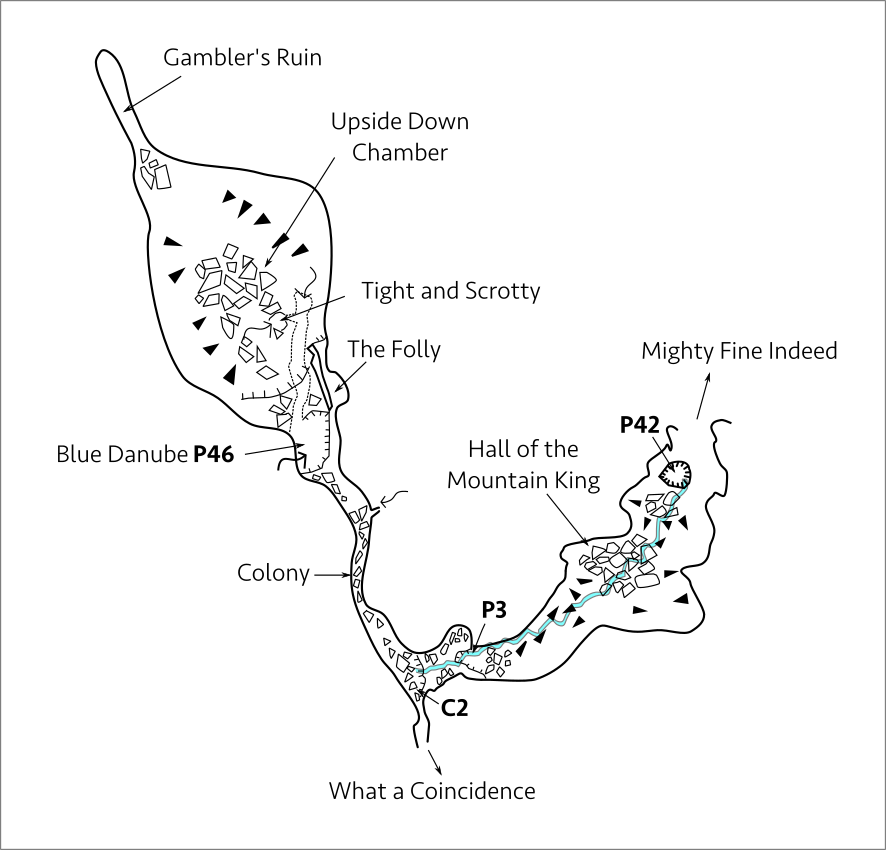
\includegraphics[width = \textwidth]{images/little_insets/upside_down.png}}
\caption{Upside Down Chamber} \label{map: upside down}
\end{survey}

I scampered up the slope waiting for Arun to join me. We wandered round in awe.\sidenote{\passage{Upside Down Chamber} is likely the third largest chamber in the system.} In my wanderings I nearly stepped on something. A dead bat! And not too long dead given the amount of organic matter around it (though it's hard to tell in the cold and relatively sterile environment of the cave). This leads to a pun making session that lasts for the best part of an hour to attempt to name this place but we don't find anything that satisfying. In the end we settle on `\passage{Upside Down Chamber}'. Partly due to to the bat and partly due to the strange mud pattern on the boulders that almost makes you believe they were flipped upside down at some point in the past.

We checked out the leads. At the bottom of the chamber, under the boulders, there is some water dripping down. It seems possible to follow it but it'd be wet. We graciously leave that for a future explorer. At the top of the boulder slope is a rift heading into the wall. It's odd, like a fault, not something formed by water. Its very tight, but there's a human sized slot heading downwards so I placed a couple of bolts and descend. The rift goes down maybe 15 metres, and I needed to place two rebelays to avoid the perilously sharp rock. At the bottom, in a small enlargement it doesn't seem like there's any way on, so we head back out derigging as we go. 

Back in the chamber, looking at the same rift it looks like you can climb up to a ledge. Perhaps there'll be a way above the constriction and it will open out we thought. The only problem is we don't have bolt climbing kit. But I can see a way up. A ledge of rock a few metres from the rift can be climbed on. From there a sideways traverse will get you onto the bottom of a slope which it should be possible to carefully climb up into the rift and to the ledge above. 

Arun seems happy to let me do the traverse. I place a couple of bolts back on the wall and the, roped up lean out across the wall. I place a bolt as far away as I can and attach the rope to it, then clip into it and the rope. I swung over and dangled on it, now nearly a metre closer to my goal. I repeated this a few times. Bolt, rope, swing. Mounting the slope was trickier than I thought, trailing the drill bag and the rope behind me, but \bignote{fear is a great motivator} and I was soon climbing a less exposed section. A couple of metres up I found myself on the ledge. I put a a bolt in to finish my epic traverse. At the top, as is so often the case, there was only disappointment the rift was completely closed up here and looking backwards into the chamber the ceiling was high high above and there were no windows anywhere near. A thoroughly useless climb. 


Back down. Derigging was as precarious as rigging but it's probably best left to the imagination. Arun and I were sated by our few hours in the chamber so began our long journey out. On the way up Arun unleashed a huge volume of rocks that I was lucky enough to avoid and we were within audible range of Jack when Kenneth dropped a drill on his head. There's never a dull moment in \passage{Primadona}.

\name{Rhys Tyers}


